% Opcje klasy 'iithesis' opisane sa w komentarzach w pliku klasy. Za ich pomoca
% ustawia sie przede wszystkim jezyk oraz rodzaj (lic/inz/mgr) pracy.
\documentclass[shortabstract]{iithesis}

\usepackage[utf8]{inputenc}

%%%%% DANE DO STRONY TYTUŁOWEJ
% Niezaleznie od jezyka pracy wybranego w opcjach klasy, tytuł i streszczenie
% pracy nalezy podac zarowno w jezyku polskim, jak i angielskim.
% Pamietaj o madrym (zgodnym z logicznym rozbiorem zdania oraz estetyka) recznym
% złamaniu wierszy w temacie pracy, zwlaszcza tego w jezyku pracy. Uzyj do tego
% polecenia \fmlinebreak.
\polishtitle    {Aplikacja webowa do obsługi\fmlinebreak rozgrywek tenisowych}
\englishtitle   {English title}
\polishabstract {Celem pracy jest zaprojektowanie i stworzenie aplikacji webowej umożliwiającej organizację rozgrywek tenisa ziemnego. Projekt obejmuje opracowanie responsywnego interfejsu użytkownika wraz z zapleczem. Każdy element aplikacji został skonteneryzowany i skonfigurowany do współpracy z resztą projektu. }
\englishabstract{TODO streszczenie po angielsku \ldots}
% w pracach wielu autorow nazwiska mozna oddzielic poleceniem \and
\author         {Marcin Wróbel}
% w przypadku kilku promotorow, lub koniecznosci podania ich afiliacji, linie
% w ponizszym poleceniu mozna zlamac poleceniem \fmlinebreak
\advisor        {dr hab. Dariusz Biernacki}
%\date          {}                     % Data zlozenia pracy
% Dane do oswiadczenia o autorskim wykonaniu
\transcriptnum {323830}                     % Numer indeksu
\advisorgen    {dr hab. Dariusza Biernackiego} % Nazwisko promotora w dopelniaczu
%%%%%

%%%%% WŁASNE DODATKOWE PAKIETY
%
\usepackage{float,dirtree}
% \usepackage{graphicx,listings,amsmath,amssymb,amsthm,amsfonts,tikz}
\usepackage{graphicx,listings,amsmath}
%
%%%%% WŁASNE DEFINICJE I POLECENIA
%
%\theoremstyle{definition} \newtheorem{definition}{Definition}[chapter]
%\theoremstyle{remark} \newtheorem{remark}[definition]{Observation}
%\theoremstyle{plain} \newtheorem{theorem}[definition]{Theorem}
%\theoremstyle{plain} \newtheorem{lemma}[definition]{Lemma}
%\renewcommand \qedsymbol {\ensuremath{\square}}
% ...
%%%%%

\begin{document}

%%%%% POCZĄ„TEK ZASADNICZEGO TEKSTU PRACY

\chapter{Wprowadzenie}
Obsługa amatorskich lig tenisa ziemnego bardzo często polega na wykorzystaniu notesu i długopisu.
W ramach tych lig zawodnicy są zazwyczaj zobowiązani do własnej organizacji meczów i pozyskiwania danych kontaktowych innych uczestników w celu ustalenia terminów spotkań.
Pojawiła się potrzeba stworzenia nowoczesnego narzędzia do organizacji amatorskich rozgrywek ligowych.
W poniższej pracy przedstawiono aplikację webową, która odpowiada na tę potrzebę.
\par
Aplikacja umożliwia łatwe wprowadzanie wyników meczów, weryfikuje je oraz uwzględnia przypadki szczególne, takie jak walkover, czy krecz.
Na podstawie wyników meczów sytuacja w grupie i drabince turniejowej jest obliczana automatycznie.
Zawodnicy mają dostęp do danych kontaktowych osób, z którymi mają rozegrać mecz i są powiadamiani o zakończonych meczach i zmianach w tabeli.
Aplikacja udostępnia także bogatą parametryzację, pozwalającą dostosować system do wymagań danej rozgrywki.

\par
Co istotne, dzięki responsywnemu interfejsowi użytkownika, aplikacja jest przystosowana zarówno do urządzeń mobilnych, jak i stacjonarnych,
Dzięki temu zawodnicy mają możliwość korzystania z systemu nie tylko w domu, ale również w przerwach w pracy, czy na korcie tenisowym.
Aplikacja webowa została opublikowana i jest dostępna na stronie \texttt{www.rozgrywkitenisa.pl}.
\par

\chapter{Opis zagadnienia}
Na początku projektu zaimplementowane zostały tylko podstawowe funkcjonalności. Z czasem zostały dokładane nowe pomysły
i ostatecznie zrealizowano następujące funkcjonalności:
\begin{itemize}
    \item Tworzenie rozgrywek, faza grupowa jest opcjonalna
    \item Liczba grup i zawodników w fazie pucharowej jest konfigurowalna.
          W pojedynczej rozgrywce liczba zawodników została ograniczona do 128, a liczba grup została ograniczona do 24.
          Limity zostały wybrane arbitralnie i mogą zostać zmienione.
          Niestety limity są konieczne ponieważ nie można pozwolić użytkownikowi na stworzenie rozgrywki o bardzo dużej (np. 10000) liczbie grup, lub zawodników.
          Przeglądarka nie potrafiłaby ich wyrenderować.
    \item Podczas tworzenia rozgrywki skład grup jest losowany. Losowanie jest wspomagane rankingiem.
          W przypadku rozgrywek bez fazy grupowej rozstawienie zawodników w fazie pucharowej ustalane jest na podstawie rankingu.
    \item Zawodnicy mają dostęp do danych kontaktowych osób, z którymi będą rozgrywać mecz.
    \item Wynik meczu może wpisywać organizator/sędzia, lub zawodnicy.
    \item Wynik meczu obsługuje przypadki szczególne:
          \begin{itemize}
              \item walkower - w tabeli wynik liczony jest tak jakby zawodnik poddający się przegrał wszystkie gemy, aż do zwycięstwa w meczu drugiego zawodnika,
              \item krecz - w tabeli wynik liczony jest tak jakby zawodnik poddający się przegrał wszystkie gemy od momentu wycofania się, aż do zwycięstwa w meczu drugiego zawodnika.
          \end{itemize}
    \item Rejestracja użytkowników. Hasło można zresetować za pomocą emaila podenego podczas rejestracji.
    \item Obliczanie rankingu na podstawie wyników zakończonych rozgrywek.
\end{itemize}
\section{Generowanie grup}
Podczas generowania grup zawodnicy są dzieleni na koszyki według rankingu.
Dla rozgrywki o $N$ zawodnikach i $M$ grupach w pierwszym koszyku znajduje się $M$ zawodników o najlepszym rankingu, w drugim koszyku kolejne $M$ zawodników, itd.
Wyjątkiem jest ostatni koszyk. Jeżeli $N \not\equiv 0 \pmod{M}$, wtedy liczba zawodników w ostatnim koszyku jest mniejsza, wynosi $N\bmod{M}$.
\section{Generowanie drabinki fazy pucharowej}
Na początku generowania drabinki fazy pucharowej zawodnicy są sortowani. Jeżeli rozgrywka posiada fazę grupową, to kolejność zależy od wyników w grupie.
Największe znaczenie ma pozycja w grupie, potem bilans meczów, bilans setów, a na końcu bilans gemów.
Jeżeli rozgrywka składa się tylko z fazy pucharowej to kolejność zawodników zależy od pozycji w rankingu ogólnym.

Posortowanym zawodnikom przypisane zostają numery startowe od $0$ do $N-1$, gdzie $N$ to ilość zawodników.
Numery startowe są następnie przypisywane do drabinki według poniższego algorytmu. Jego wizualizacja znajduje się na rysunku~\ref{fig:knockout_bracket_generation}.
\begin{lstlisting}
    numeryStartowe=[0,1]
    dopoki (numeryStartowe.rozmiar() < N) {
        poprzednieNumeryStartowe = numeryStartowe
        numeryStartowe = []
        najwiekszyNumer = poprzednieNumeryStartowe.rozmiar() * 2 - 1
        dla kazdego (ns w poprzednieNumeryStartowe) {
            numeryStartowe.dodaj(ns)
            numeryStartowe.dodaj(najwiekszyNumer - ns)
        }
    }
    zwroc numeryStartowe
\end{lstlisting}
Kolejne pary w zwróconej liście odpowiadają kolejnym parom w drabince fazy pucharowej.
Przykładowo dla $N=8$ zostanie zwrócona lista $[0, 7, 3, 4, 1, 6, 2, 5]$. Odpowiada to parom
$[0, 7]$, $[3, 4]$, $[1, 6]$, $[2, 5]$.
\begin{figure}[H]
    \centering
    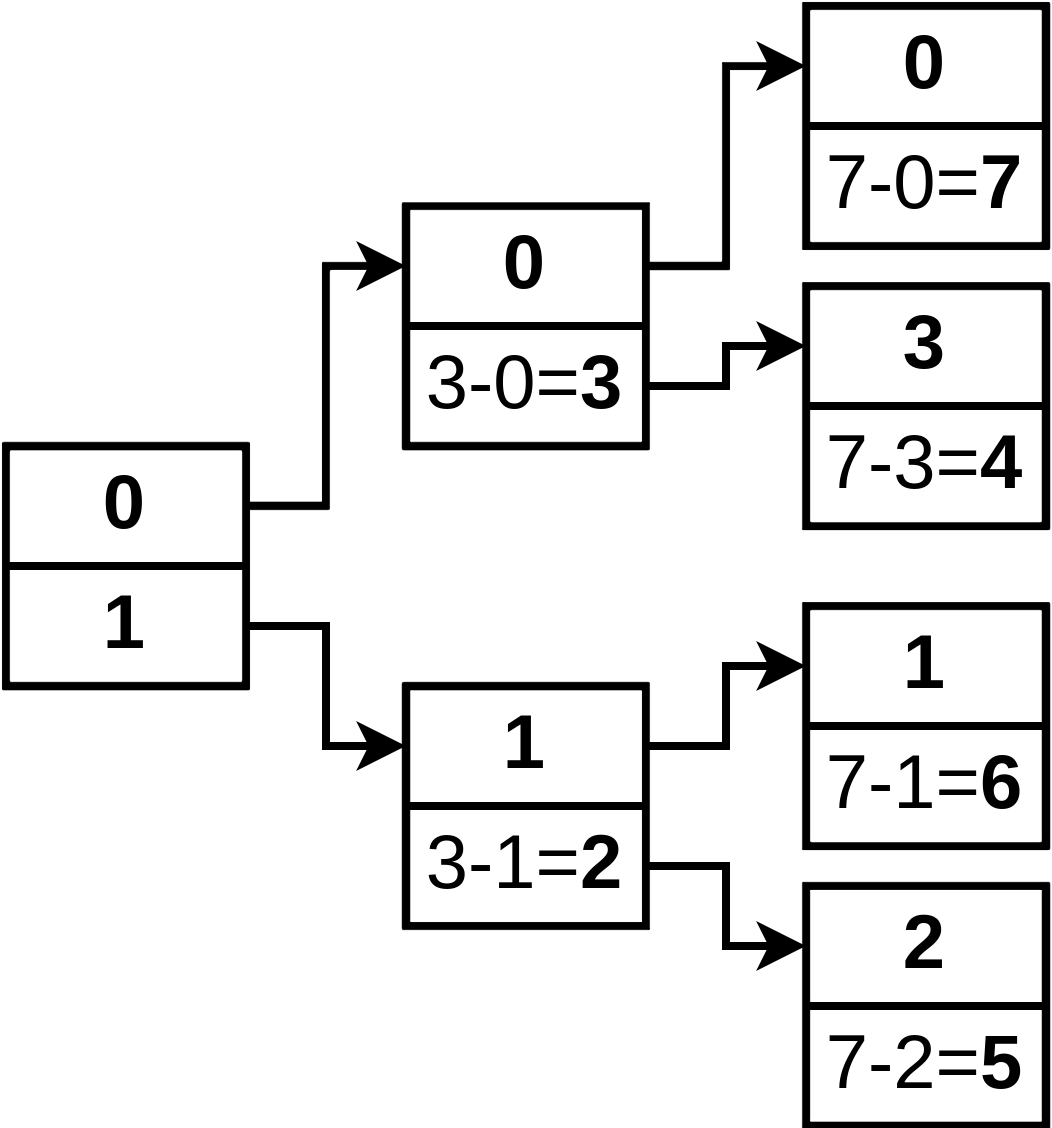
\includegraphics[width=0.5\textwidth]{assets/generowanie_drabinki.png}
    \caption{Schemat generowania drabinki fazy pucharowej}
    \label{fig:knockout_bracket_generation}
\end{figure}

\chapter{Opis aplikacji}
TODO inne sekcje opisu \ldots
\section{Instalacja}
\noindent
Aplikacja została przygotowana do uruchomienia w dwóch środowiskach:
\begin{itemize}
    \item lokalnym - do testowania na urządzeniu użytkownika,
    \item produkcyjnym - gdy aplikacja jest publicznie dostępna
\end{itemize}
Instrukcje instalacji dla środowiska lokalnego i produkcyjnego różnią się, różnice są oznaczone.
\subsection{Zmienne środowiskowe}
\noindent
Należy utworzyć pliki zawierające zmienne środowiskowe (\texttt{.env}).
Pliki \texttt{.env.example} zawierają przykładowe wartości, które pozwalają na uruchomienie w środowisku lokalnym.
\begin{itemize}
    \item
          \begin{lstlisting}[language=bash]
    cp .env.example .env
    \end{lstlisting}

    \item
          \begin{lstlisting}[language=bash]
    cd frontend
    cp .env.example .env
    \end{lstlisting}
\end{itemize}
Następnie można dostosować wartości do własnej konfiguracji.


\subsection{Instalacja zależności}
Aby zbudować i uruchomić projekt należy zainstalować \texttt{Docker} zgodnie z instrukcjami zawartymi w oficjalnej dokumentacji
\\
\url{https://docs.docker.com/}
\\
\url{https://docs.docker.com/engine/install/}
\\
Użytkownik musi należeć do grupy \texttt{docker}

\begin{lstlisting}[language=bash]
sudo usermod -aG docker nazwa_uzytkownika
\end{lstlisting}

\subsection{Budowanie}
Aby zbudować projekt należy wykonać poniższe polecenie:

\begin{lstlisting}[language=bash]
# srodowisko produkcyjne
docker compose build
# srodowisko lokalne
docker compose -f docker-compose-localhost.yml build
\end{lstlisting}

\subsection{Uruchamianie}
\begin{lstlisting}[language=bash]
# srodowisko produkcyjne
docker compose up -d
# srodowisko lokalne
docker compose -f docker-compose-localhost.yml up -d
\end{lstlisting}
Flaga \texttt{-d} nie jest wymagana, uruchamia projekt w tle.

\subsection{Wyłączanie}
\begin{lstlisting}[language=bash]
docker compose down
\end{lstlisting}

\chapter{Architektura aplikacji}
\section{Struktura aplikacji}
Aplikacja została podzielona na 5 głównych części:
\begin{itemize}
    \item \textbf{frontend} - cześć aplikacji widoczna dla użytkownika
    \item \textbf{backend} - odpowiada za przekazywanie i odbieranie danych od frontendu, odczytuje i zapisuje dane do bazy danych
    \item \textbf{baza danych} - przechowuje dane aplikacji
    \item \textbf{reverse proxy} - wysyła, odbiera, przekazuje zapytania do odpowiednich części aplikacji
    \item \textbf{narzędzie do odnawiania certyfikatów SSL/TLS} - automatyzuje proces odnawiania certyfikatów SSL/TLS
\end{itemize}
Każda część aplikacji jest opisana w następnej sekcji.
\subsection{Docker}
W celu utrzymania dobrej współpracy pomiędzy wszystkimi elementami aplikacji zdecydowałem się użyć Dockera\cite{Docker}.
Każda z 5 części aplikacji jest opakowywana w osobny kontener, czyli lekką maszynę wirtualną, która zawiera tylko potrzebne do jej działania zależności.
Konfiguracja całego środowiska znajduje się w pliku \texttt{docker-compose.yml}. Najważniejsze elementy zostały pokazane na rysunku \ref{fig:docker_containers_environment}.

\begin{figure}[H]
    \centering
    \includegraphics[width=\textwidth]{assets/środowisko_dockera.png}
    \caption{Struktura kontenerów Dockera}
    \label{fig:docker_containers_environment}
\end{figure}
\section{Kontenery Dockera}

\subsection{Reverse Proxy - Nginx}
Nginx\cite{Nginx} działa jako Reverse Proxy i jest odpowiedzialny za przekierowywanie zapytań http i https do odpowiednich części aplikacji.
W folderze \texttt{nginx/config/} znajdują się 3 pliki konfiguracyjne. Podczas działania aplikacji używany jest dokładnie jeden z nich.

\begin{itemize}
    \item \texttt{nginx\_init\_ssl\_certificate.conf} jest używany podczas pierwszego uruchomienia w środowisku produkcyjnym, obsługuje tylko zapytania http i pozwala kontenerowi Certbot(\ref{subsec:Certbot}) na pobranie certyfikatu SSL/TLS. Jest potrzebny, ponieważ nie jest możliwe obsługiwanie zapytań https bez poprawnego certyfikatu SSL/TLS.
    \item \texttt{nginx.conf} jest używany w środowisku produkcyjnym. Definiuje przekierowywanie zapytań do odpowiednich kontenerów. W tej konfiguracji nieszyfrowana komunikacja za pomocą http jest przekierowywana do szyfrowanej komunikacji za pomocą https.
    \item \texttt{nginx\_localhost.conf} jest używany w środowisku lokalnym.
\end{itemize}
\begin{figure}[H]
    \centering
    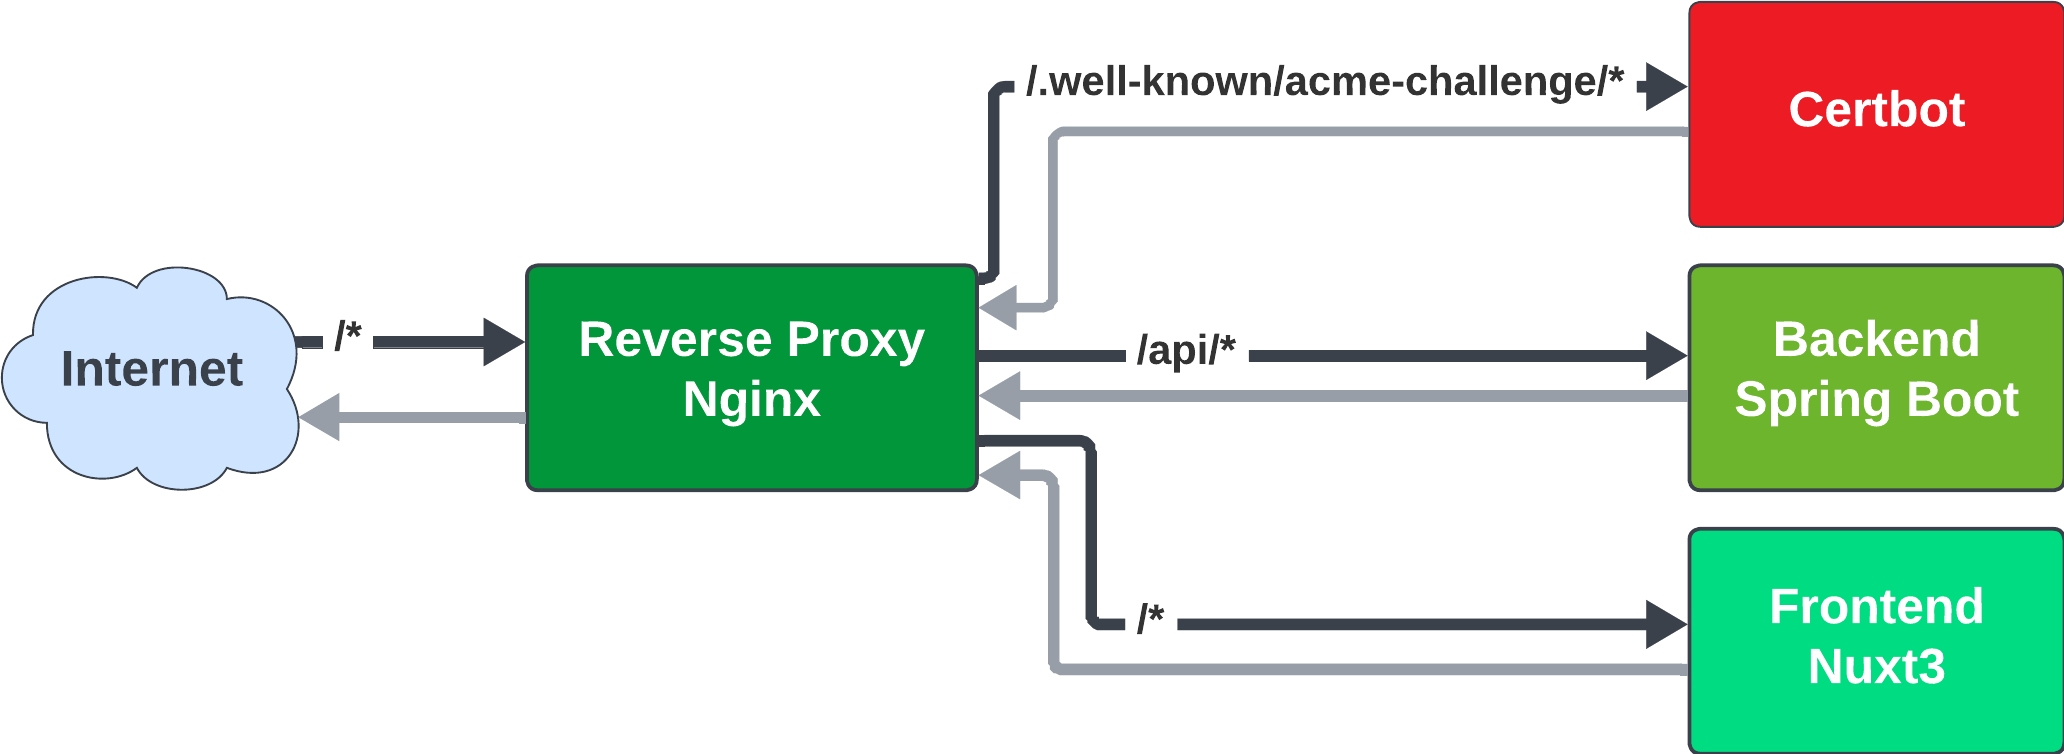
\includegraphics[width=\textwidth]{assets/przepływ_zapytań_http.png}
    \caption{Przepływ zapytań https zdefiniowanych w pliku \texttt{nginx.conf}}
    \label{fig:https_requests_flow}
\end{figure}
Na rysunku \ref{fig:https_requests_flow} pokazano schemat przepływu zapytań https dla pliku \texttt{nginx.conf}.
W przypadku zapytania http reverse proxy nie przekazuje zapytania do kolejnego kontenera, a odpowiada klientowi od razu przekierowaniem do https. Dla zapytań https zdefiniowane są następujące reguły:
\begin{enumerate}
    \item Jeżeli url zaczyna się od \texttt{/.well-known/acme-challenge/} przekaż zapytanie do kontenera Certbot.
    \item Jeżeli url zaczyna się od \texttt{/api} przekaż zapytanie do kontenera backend.
    \item W przeciwnym przypadku przekaż zapytanie do kontenera frontend.
\end{enumerate}
Wszystkie odpowiedzi na zapytania przekazywane są do reverse proxy, a reverse proxy przekazuje je dalej do nadawcy zapytania.

\subsection{Frontend - Nuxt3, Vue.js}
Frontend został napisany we frameworku Nuxt3~\cite{Nuxt3}, który oparty jest na Vue.js.
Użyłem języka TypeScript, ponieważ wprowadza on statyczne typowanie.
TypeScript w porównaniu do JavaScriptu ułatwił pisanie kodu, dzięki lepszym podpowiedziom środowiska programistycznego oraz pozwolił zapobiegać błędom, szybciej ostrzegając o problemach podczas kompilacji.
Do utrzymania jednolitego formatowania kodu źródłowego użyłem narzędzia Prettier~\cite{Prettier}.
Kod źródłowy frontendu znajduje się w folderze \texttt{frontend/}. W projekcie struktura plików frontendu oparta jest na
standardach zdefiniowanych w dokumentacji Nuxt3.
\begin{figure}[H]
    \dirtree{%
        .1 frontend.
        .2 components.
        .2 composables.
        .2 pages.
        .2 plugins.
        .2 public.
        .2 middleware.
        .2 types.
        .2 utils.
    }
    \caption{Zarys struktury plików}
\end{figure}
% W Nuxt3 struktura strony odpowiada plikom w folderze pages zgodnie z zasadami zdefiniowanymi w dokumentacji\cite{Nuxt3DocsPages}.
\noindent
Zawartość tych folderów jest następująca:
\begin{itemize}
    \item \texttt{components/} zawiera elementy interfejsu użytkownika (np. tabela wyników, element tablicy wyników, drabinka turniejowa)
    \item \texttt{composables/} zawiera elementy logiki, które posiadają swój stan i są używane w wielu miejscach. Moja aplikacja definiuje \texttt{AuthStatus}, który jest odpowiedzialny za przechowywanie informacji o tym, czy użytkownik jest zalogowany, czy nie.
    \item \texttt{pages/} struktura adresów url odpowiada plikom w tym folderze\\(np. \texttt{rozgrywkitenisa.pl/rozgrywki/123} $\longrightarrow$ \texttt{pages/rozgrywki/[id].vue})
    \item \texttt{plugins/} zawiera konfigurację dwóch pluginów (FontAwesome~\cite{FontAwesome} (dostarcza ikony aplikacji), VueDatePicker~\cite{VueDatePicker} (Dostarcza narzędzie do wybierania daty)
    \item \texttt{public/} zawiera statyczne pliki, które nie są zmieniane podczas kompilacji i~są przekazywane jako niezmienione klientowi
    \item \texttt{middleware/} zawiera middleware, które odpowiedzialne są za modyfikowanie zapytań przed przekazaniem ich dalej. Moja aplikacja używa tylko 1 middleware \texttt{logged.in.ts}, który przekierowuje niezalogowanych użytkowników do strony logowania
    \item \texttt{types/} zawiera pliki definiujące typy języka TypeScript
    \item \texttt{utils/} zawiera funkcje i stałe używane w co najmniej 2 plikach aplikacji
\end{itemize}
Oprócz wyżej wymienionych technologii zastosowałem bibliotekę TailwindCSS~\cite{TailwindCSS} do stylizacji aplikacji.
W pliku \texttt{tailwind.config.js} znajduje się konfiguracja tej biblioteki, wraz z dedykowaną dla tego projektu paletą kolorów.
Wielokrotnie używałem prefiksów dla stylów oferowanych przez TailwindCSS, które aktywują/dezaktywują dany styl w zależności od wielkości ekranu.
Dzięki temu aplikacja jest responsywna i dostosowana do komputerów i urządzeń mobilnych.


\subsection{Backend - Spring Boot}
Backend napisałem używając frameworka Spring Boot. Do zarządzania zależnościami i do automatyzacji budowania użyłem narzędzia Maven.
\\Kod backendu został podzielony na warstwy:
\begin{itemize}
    \item \textbf{kontrolery} - odpowiedzialne za przetworzenie parametrów żądania, wysłanie odpowiedzi
    \item \textbf{serwisy} - odpowiedzialne za logikę biznesową backendu
    \item \textbf{repozytoria} - odpowiedzialne za komunikację z bazą danych
\end{itemize}
Dodatkowo każdy obiekt przechowywany w bazie danych posiada klasy odpowiedzialne za ich działanie:
\begin{itemize}
    \item \textbf{encje} - definiują pola, cechy obiektu przechowywanego w bazie danych
    \item \textbf{obiekty} transferu danych (DTO) - definiują obiekty przesyłane z, lub do serwera
    \item \textbf{maper} - klasy służące do konwertowania obiektów między encjami, a obiektami transferu danych
\end{itemize}
Przykładowo dla obiektu odpowiedzialnego za rozgrywkę (\texttt{Tournament}) zdefiniowane są następujące klasy:
\begin{itemize}
    \item \texttt{TournamentController} - kontroler
    \item \texttt{TournamentMapper} - maper
    \item \texttt{TournamentRepository} - repozytorium
    \item \texttt{TournamentService} - serwis
    \item \texttt{Tournament} - encja
    \item \texttt{TournamentCreateDto} - obiekt transferu danych wysyłany przez frontend podczas żądania stworzenia rozgrywki
    \item \texttt{TournamentBasicDto} - obiekt transferu danych zawierający tylko podstawowe informacje o rozgrywce, jest używany podczas wysyłania listy wszystkich rozgrywek
\end{itemize}

\subsection{Baza danych - PostgreSQL}
Do przechowywania danych wybrałem PostgreSQL.
Zdecydowałem się wybrać tą technologię ze względu na to, że chciałem użyć relacyjnej bazy danych, która jest wydajna, niezawodna i aktywnie rozwijana. PostgreSQL spełnia wszystkie te wymagania.
\par
Konfiguracja bazy danych jest zarządzana przez backend i narzędzie Flyway~\cite{Flyway}.
W~folderze \texttt{backend/src/main/resources/db/migration} znajdują się pliki z poleceniami SQL definiujące migracje pomiędzy wersjami.
Gdy schemat bazy danych był zmieniany dokładałem kolejny plik odpowiedzialny za migrację. Przy uruchomieniu backendu Flyway automatycznie sprawdza, czy zostały dodane jakieś pliki migracyjne.
Jeżeli tak, to dokonuje migracji.
Dzięki temu baza danych używana lokalnie oraz baza danych na serwerze w wersji produkcyjnej utrzymują ten sam schemat bazy danych.

\subsection{Narzędzie do odnawiania certyfikatów SSL/TLS - Certbot}
Dla bezpieczeństwa użytkowników połączenie z stroną internetową powinno być szyfrowane.
Do nawiązania szyfrowanego połączenia używane są certyfikaty SSL/TLS, które zawierają klucz publiczny i inne dane, takie jak okres ważności, dane właściciela, wystawcy.
Każdy ma możliwość wystawić własny certyfikat, ale przeglądarka będzie ufać tylko certyfikatom wydanym przez zaufane (według twórców przeglądarki) instytucje.
Świadomy użytkownik znając wystawcę certyfikatu może ręcznie dodać go do listy zaufanych certyfikatów. Takie rozwiązanie jest właściwe tylko wtedy, gdy nie chcemy powierzać generowania kluczy zewnętrznej instytucji i użytkownicy mogą potwierdzić jego prawdziwość (np. gdy wystawiamy certyfikat aplikacji webowej do użytku wewnętrznego firmy).
W związku z tym, że aplikacja webowa będąca tematem pracy będzie publicznie dostępna, generowanie certyfikatów SSL/TLS powierzyłem organizacji Let's Encrypt~\cite{LetsEncrypt}.
Let's Encrypt wystawia darmowe certyfikaty SSL/TLS oraz umożliwia automatyzację tego procesu.
Kontener Certbot oparty jest na narzędziu o tej samej nazwie~\cite{Certbot}.
Odpowiada on za automatyczne odnawianie certyfikatów poprzez wysyłanie zapytania do Let's Encrypt i odpowiadanie serwerom tej organizacji na zapytania weryfikujące - czy prośbę o~wydanie certyfikatu wysłał właściciel domeny rozgrywkitenisa.pl.

\label{subsec:Certbot}

%%%%% BIBLIOGRAFIA

\begin{thebibliography}{1}
    \bibitem{Docker} Dokumentacja Dockera, \url{https://docs.docker.com/}
    \bibitem{Nginx} Dokumentacja Nginx, \url{https://docs.nginx.com/}
    \bibitem{Nuxt3} Nuxt3, \url{https://nuxt.com/}
    \bibitem{Prettier} Prettier \url{https://prettier.io/}
    \bibitem{Nuxt3DocsPages} Nuxt3 - dokumentacja struktury plików w folderze pages/, \url{https://nuxt.com/docs/guide/directory-structure/pages}
    \bibitem{FontAwesome} FontAwesome \url{https://fontawesome.com/docs}
    \bibitem{VueDatePicker} VueDatePicker \url{https://vue3datepicker.com/}
    \bibitem{TailwindCSS} TailwindCSS \url{https://tailwindcss.com/}
    \bibitem{SpringBoot} SpringBoot \url{https://spring.io/projects/spring-boot/}
    \bibitem{Flyway} Flyway \url{https://flywaydb.org/}
    \bibitem{Certbot} Certbot \url{https://certbot.eff.org/}
    \bibitem{LetsEncrypt} LetsEncrypt \url{https://letsencrypt.org/pl/}
\end{thebibliography}

\end{document}